\documentclass[fontset=windows]{article}
\usepackage[margin=1in]{geometry}%设置边距,符合Word设定
\usepackage{ctex}
\usepackage{setspace}
\usepackage{lipsum}
\usepackage{graphicx}%插入图片
\graphicspath{{Figures/}}%文章所用图片在当前目录下的 Figures目录

\usepackage{hyperref} % 对目录生成链接,注:该宏包可能与其他宏包冲突,故放在所有引用的宏包之后
\usepackage{amsmath}
\usepackage{mathtools}
\usepackage{marginnote}
\usepackage{tcolorbox}
\usepackage{enumitem}

\hypersetup{colorlinks = true,  % 将链接文字带颜色
	bookmarksopen = true, % 展开书签
	bookmarksnumbered = true, % 书签带章节编号
	pdftitle = 基于图像的三维重建学习笔记, % 标题
	pdfauthor =Gukazma} % 作者
\bibliographystyle{plain}% 参考文献引用格式

\renewcommand{\contentsname}{\centerline{Contents}} %经过设置word格式后,将目录标题居中


\title{\heiti\zihao{2} 基于图像的三维重建学习笔记}
\author{\songti Gukazma}
\date{\today}


\begin{document}
	\maketitle
	\thispagestyle{empty}

\begin{abstract}
	基于图像的三维重建学习笔记,附个人学习批注,并详细推导计算过程。
\end{abstract}

\tableofcontents

\section{特征提取及匹配}
\subsection{特征提取}
\subsubsection{Harris角点检测}

\begin{flalign*}
&& E(u, v) &= \sum_{(x,y)}^{} w(x,y)[I(x+u,y+v)-I(x,y)]^2 &&  \\
\text{对}I(x+u,y+v)\text{一阶泰勒展开} && &\approx \sum_{(x,y)}^{} w(x,y)[I(x,y)+\frac{\partial I}{\partial x}(x,y)u +\frac{\partial I}{\partial y}(x,y)v-I(x,y)]^2 &&\\
 && &= \begin{bmatrix}u \\v\end{bmatrix}^T \mathbf{H} \begin{bmatrix}u \\v\end{bmatrix} 
&&
\end{flalign*}
\begin{tcolorbox}
二元函数函数一阶泰勒展开推导:
\begin{flalign*}
f(x,y) &\approx f(x_0,y_0) + f_{x}'(x_0,y_0)(x-x_0)	+ f_{y}'(x_0,y_0)(y-y_0)\\
\text{令$x=x+u,y=y+v$:}\\ 
f(x+u,y+v) &\approx f(x_0,y_0) + f_{x}'(x_0,y_0)(x+u-x_0)+f_{y}'(x_0,y_0)(y+v-y_0)\\
\text{令$x_0=x,y_0=y$:}\\ 
&= f(x,y) + f_{x}'(x,y)(x+u-x)+f_{y}'(x,y)(y+v-y)\\
&= f(x,y) + f_{x}'(x,y)u+f_{y}'(x,y)v
\end{flalign*}
\end{tcolorbox}

其中$\mathbf{H}$为Harris矩阵:
\begin{equation*}
H=
\begin{bmatrix}
	\sum_{(x,y)}^{}w(x,y)(\frac{\partial I}{\partial x}(x,y))^2 & \sum_{(x,y)}^{}w(x,y)(\frac{\partial I}{\partial x}(x,y)\frac{\partial I}{\partial y}(x,y)) \\
	\sum_{(x,y)}^{}w(x,y)(\frac{\partial I}{\partial y}(x,y)\frac{\partial I}{\partial y}(x,y)) & \sum_{(x,y)}^{}w(x,y)(\frac{\partial I}{\partial y}(x,y))^2
\end{bmatrix}
\end{equation*}

\begin{figure}[h]
    \centering
    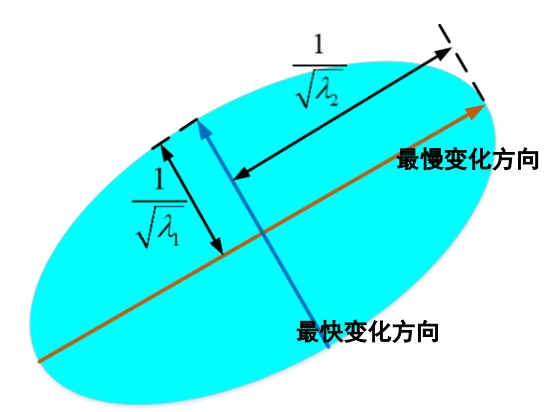
\includegraphics[height=2in]{harrisShape.png}
    \caption{Harris矩阵特征椭圆形}
    \label{fig:harrisShape}
\end{figure}

Harris 矩阵H的特征值分析:
\begin{equation*}
	SVD(H) = U \sum V, (\lambda_1, \lambda_2), \lambda_1 > \lambda_2
\end{equation*}
\begin{itemize}[leftmargin=2cm]
	\item $\lambda_1 \approx \lambda_2$ 兴趣点位于光滑区域;
	\item $\lambda_1 > 0  \lambda_2 \approx 0$ 兴趣点位于边缘区域;$\lambda_1 > 0  \lambda_2 \approx 0$ 兴趣点位于边缘区域;
	\item $\lambda_1, \lambda_2 > 0$ 兴趣点位于角点区域。
\end{itemize}

Harris角点准则:
\begin{equation*}
	C = det(H) - ktrac(H)^2 = \lambda_1\lambda_2 - k(\lambda_1 + \lambda_2)^2, k = 0.04
\end{equation*}
\begin{itemize}[leftmargin=2cm]
	\item k的值越小, 检测子越敏感
	\item 只有当$\lambda_1$和$\lambda_2$同时取得最大值时,C才能取得最大值
	\item 避免了特征值分解,提高检测效率
\end{itemize}
这里使用非极大值抑制(Non-maximal Suppression)
选取局部响应最大值,避免重复的检测。
\bibliography{books}
\end{document}